% ITEX root = ../thesis.tex
\subsection{Cauchy Distribution}
\begin{wrapfigure}{r} {0.7\textwidth}
    \begin{center}
        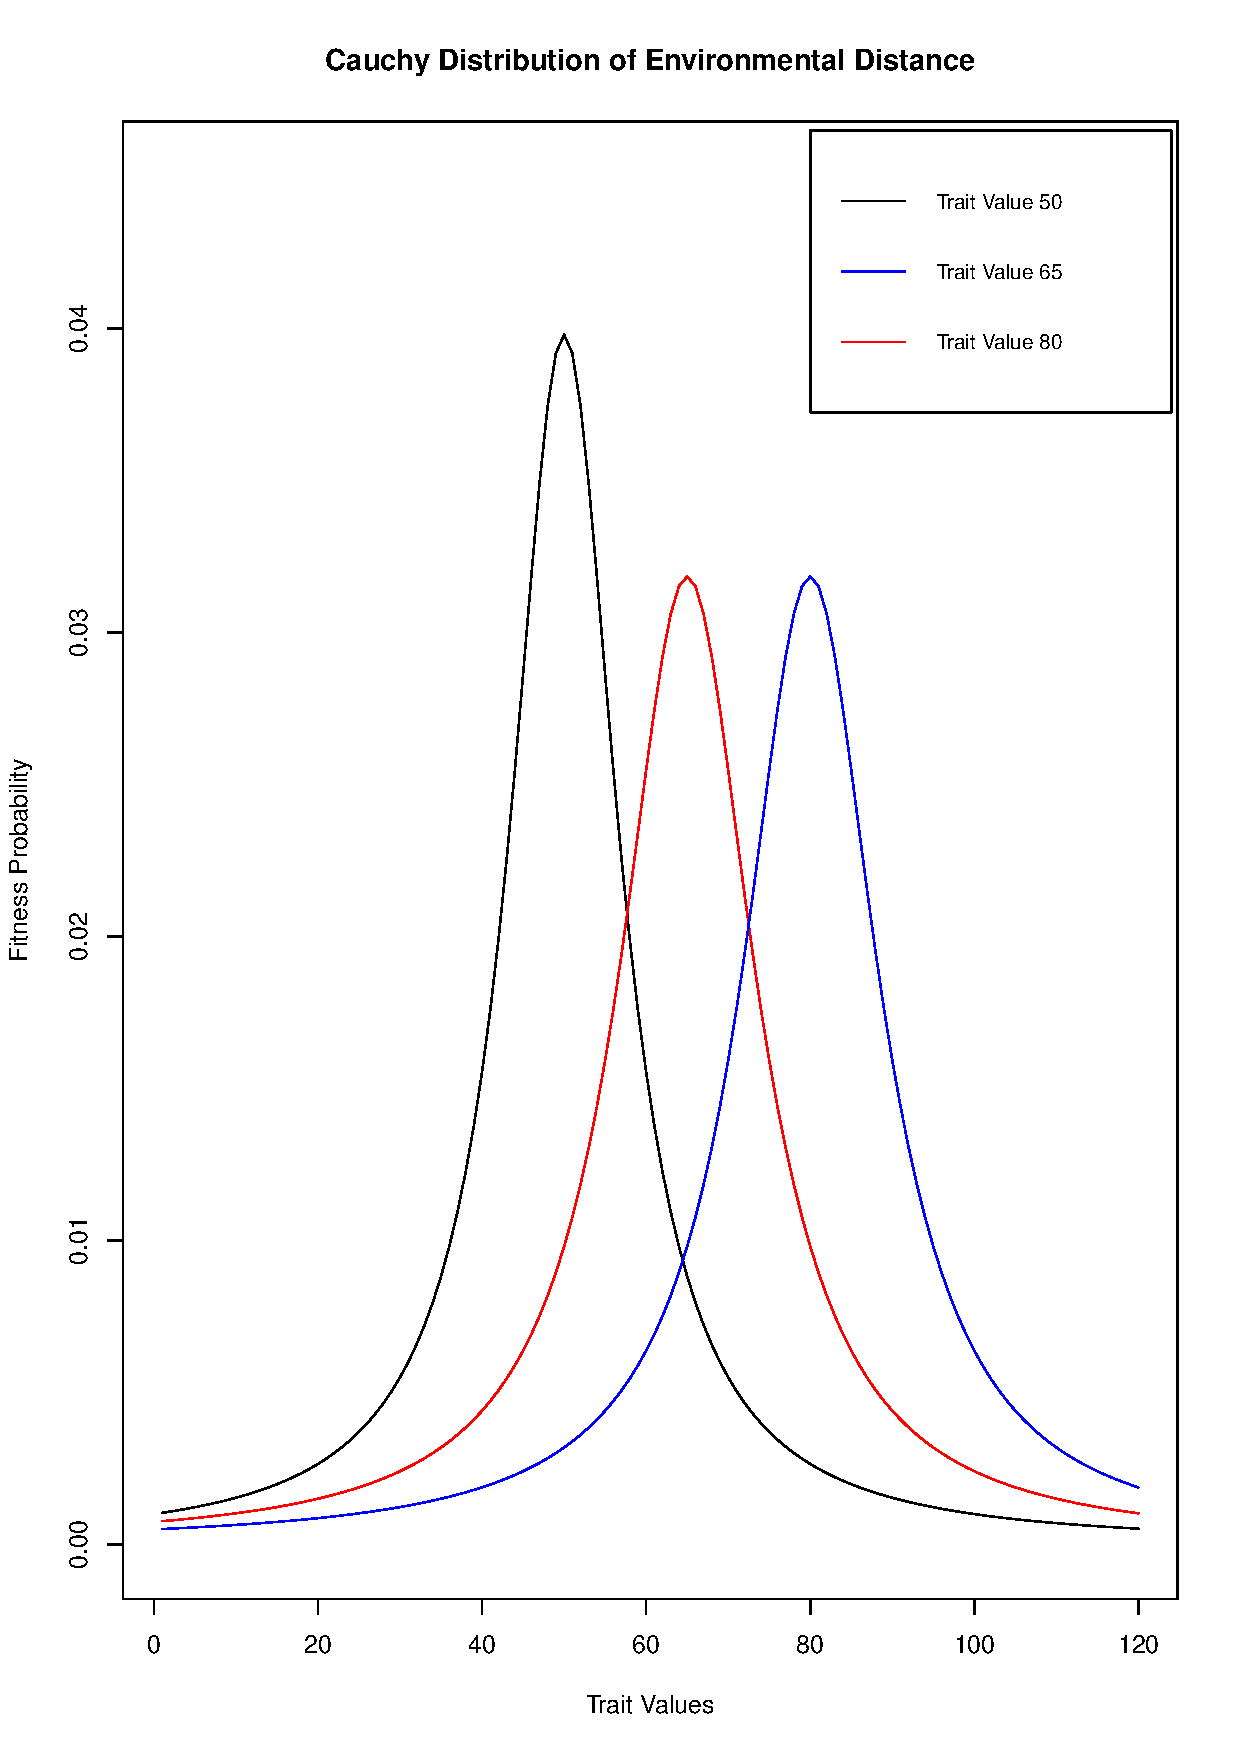
\includegraphics[scale=0.2]{../Results/Cauchy_Distribution.pdf}
    \end{center}
    \caption{Plot of the Cauchy Distribution used to derive fitness probabilities (for reproduction) and fitness values (normalising) of individuals. Distribution is also representative of the environmental distances respective populations evolved to. The main population (black) evolved to a trait value of 50, where the peak trait value has a reproductive probability of 3.98\%. Migrant populations either evolved to a trait value of 65 (blue) or 80 (red).}
    \label{fig:Cauchy Distribution}
\end{wrapfigure}

\textit{Figure 2} on the shows how the trait values are distributed along a Cauchy distribution. These desired trait values represent the environment and the distance between them is the environmental distance. The values must not be too far apart that the probability is 0, meaning that migrant genes are passed on to future generations and we see how the network develops with invading alleles. Since the Cauchy distribution is long tailed, this allowed for varying alleles to potentially persist in the population, as seen from the probability values along the y-axis.
\subsection{No Migration}
\begin{figure}[h!]
    \centering
        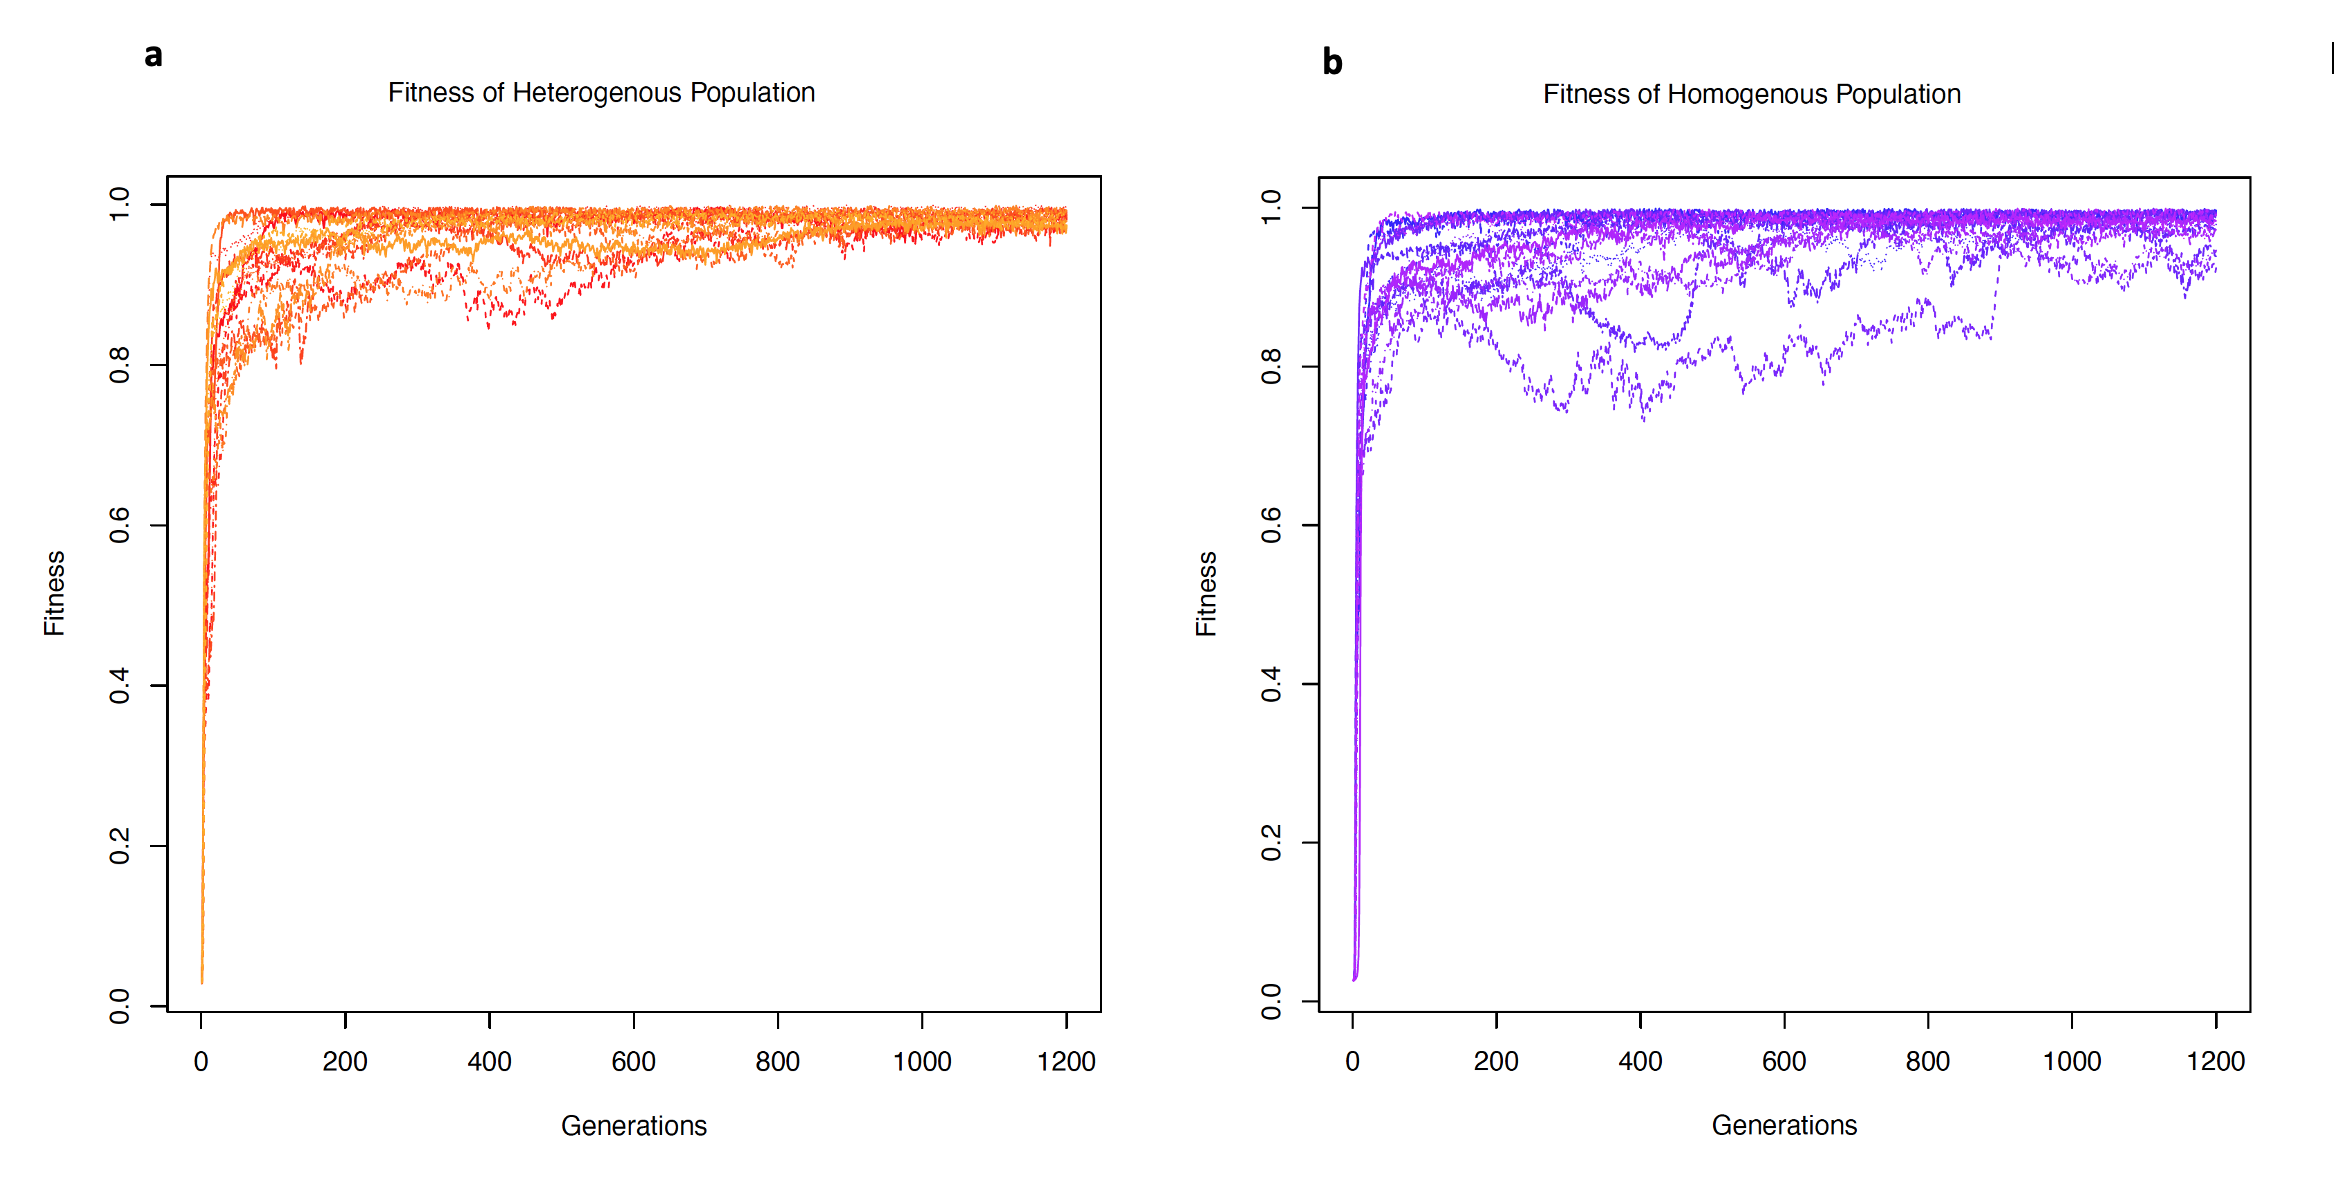
\includegraphics[width=0.9\textwidth]{../Results/no_migration.jpg}
    \caption{graphs showing the fitness evolution without migration for two different starting genetic makeups. (a) shows the evolution of a network that is homogenous network, where all starting allele values range between 0.10 and 0.30. (b) shows how a heterogenous network evolves where starting values for each allele are generated using a uniform distribution between 0.1 and 0.3. For the heterogenous populations, they had a mean fitness of 0.961, standard deviation of 0.03 while the homogenous populations had an average fitness value of 0.955 with a standard deviation of 0.05.}
    \label{fig:No Migration}
\end{figure}
When there is no migration happening, the genetic network evolves rapidly to the desired trait value. In a very short time period, it reaches an average fitness of 0.919. This can be seen from \textit{figure 3} to the right. After normalising the fitness, once the trait values of individuals however around 50, the fitness staggered close to maximum fitness, sometimes going below. When plotting the average fitness values of homogenous and heterogenous, they both show rapid evolution and have very similar patterns. Furthermore, this is seen in \textit{figure 6} which is a boxplot showing the distribution of the number of generations needed to reach the average fitness for with and without migration. It quickly rises to around 0.90 and slowly plateaus, stabilising close to 1.00, highest possible fitness. No migration overall resulted in a high average fitness, with a value of 0.958 and standard deviation of 0.04.
\subsection{Migration}
\begin{figure}[h!]
    \centering
        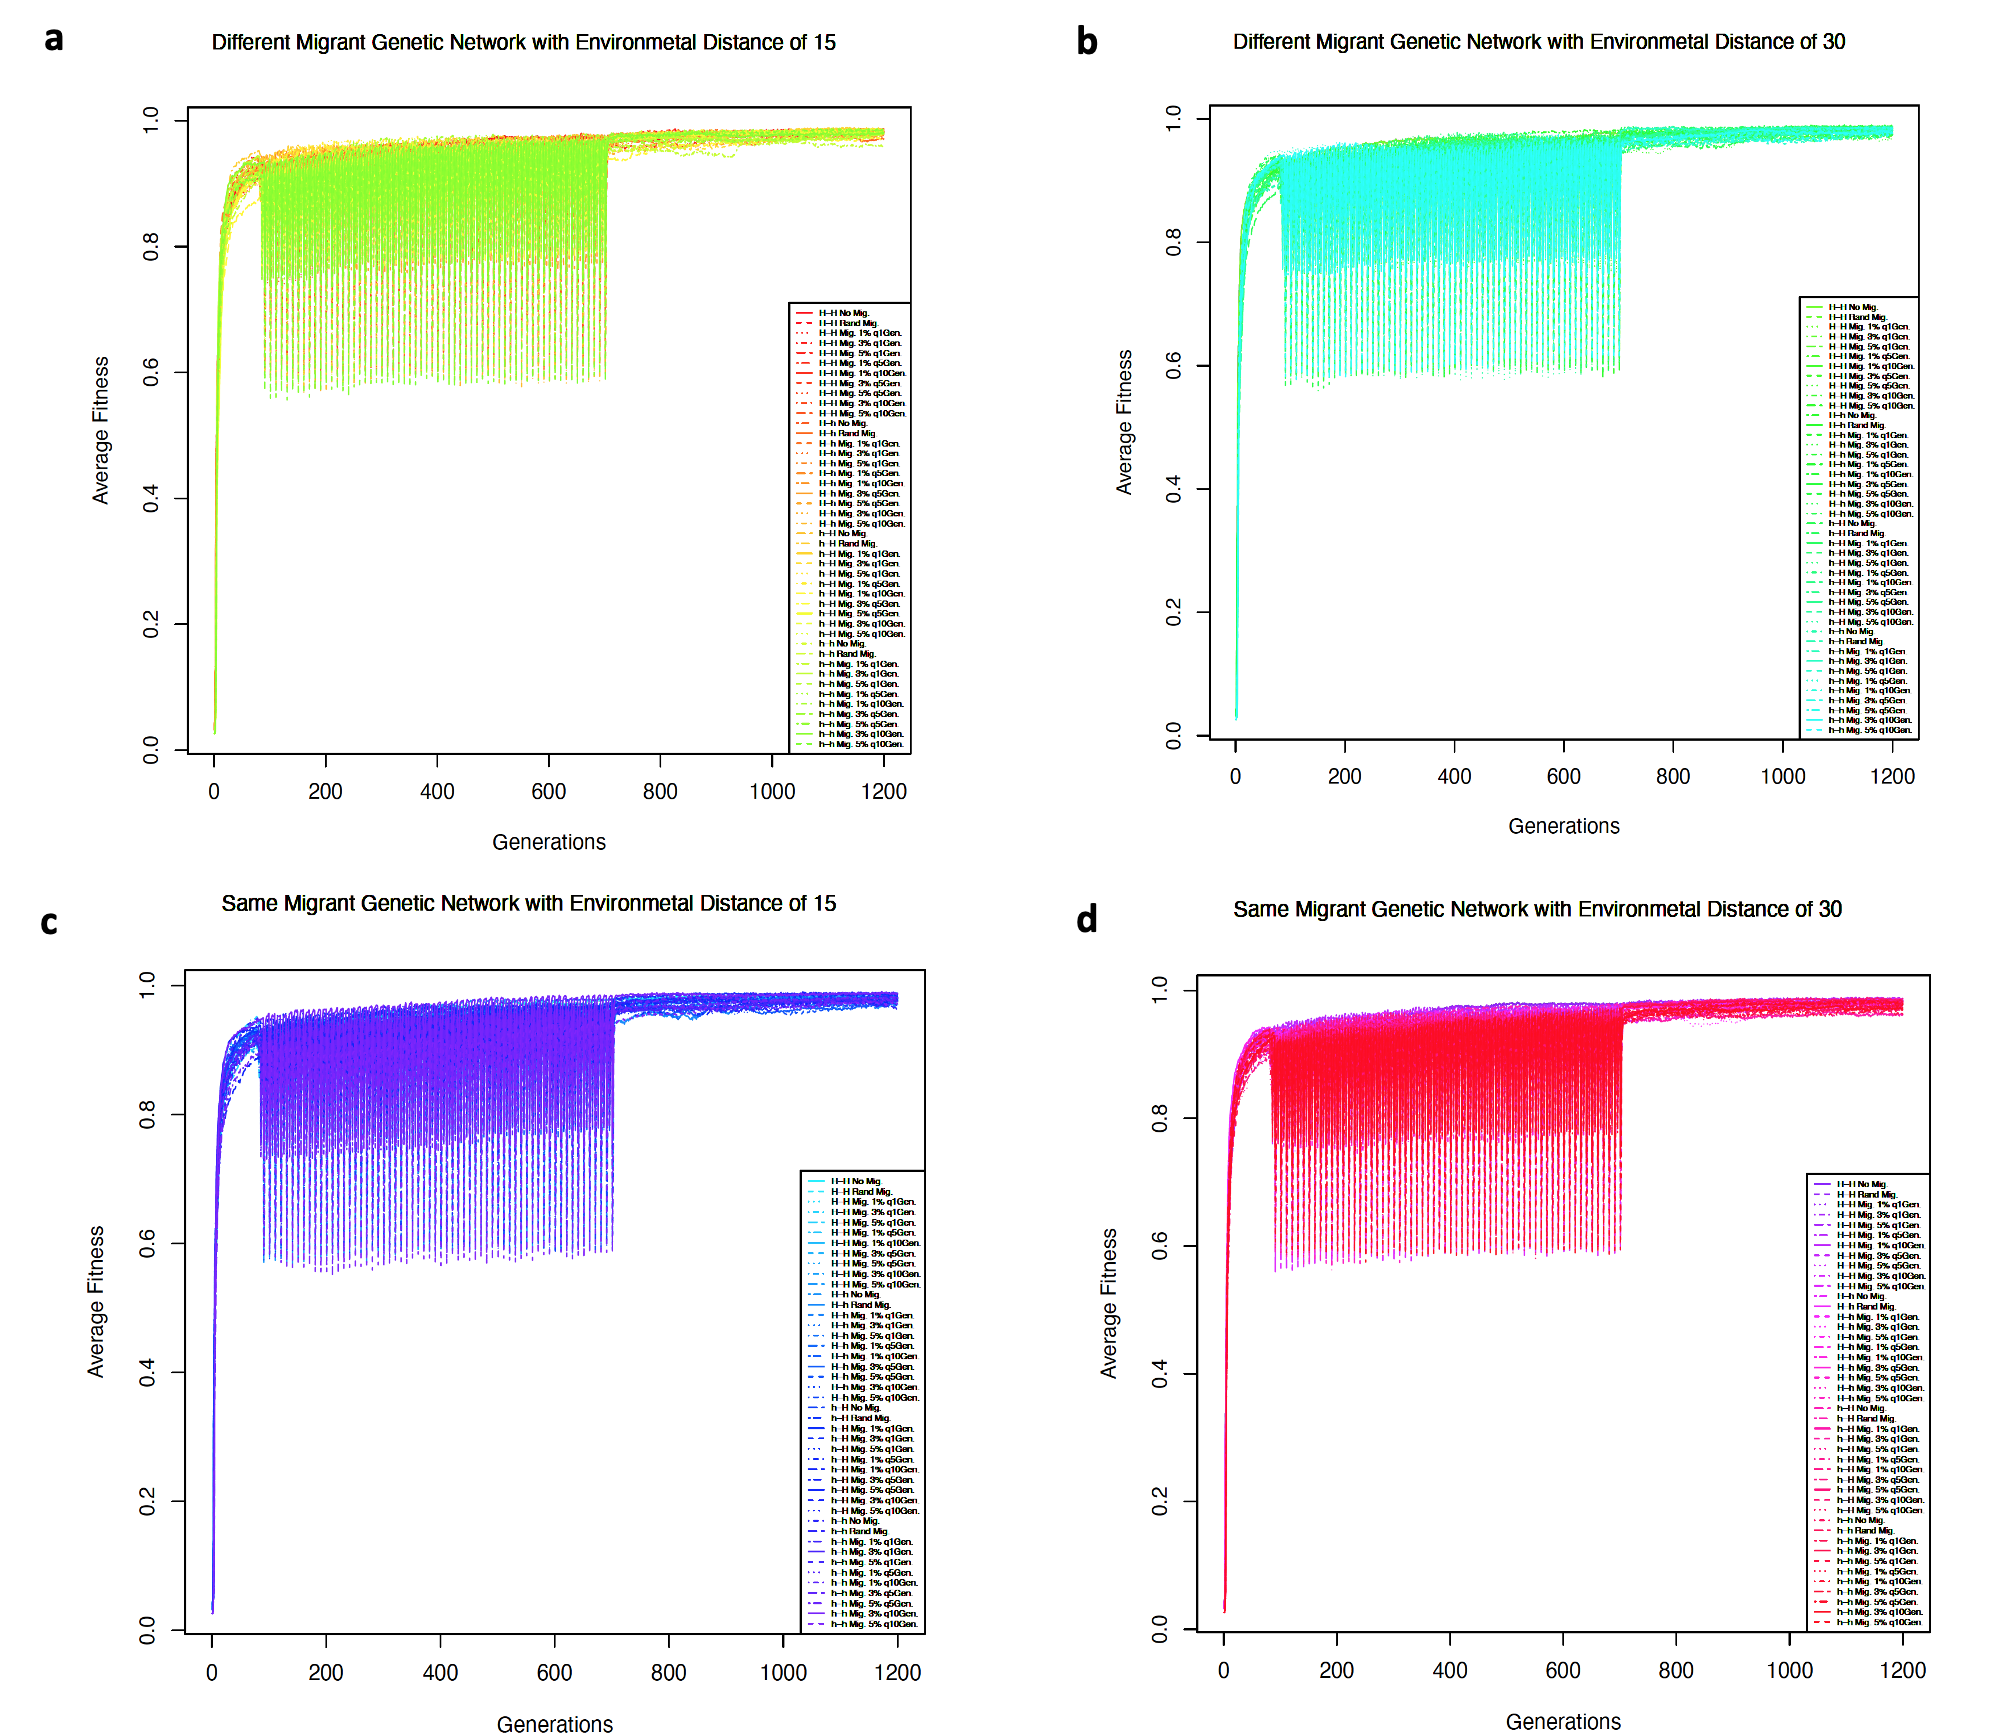
\includegraphics[width=0.9\textwidth]{../Results/migration.jpg}
    \caption{Plots showing the effect of migration on fitness over time. Migration occurs between generations 80 and 700, where the network gets 500 generations afterwards to try and recover. The graphs show how migration caused fluctuations in fitness values (a) shows the effect of migrant network with different regulations from the main population, evolving to a trait value of 65 (Environmental Distance of 15). It is a variation where gene $y_1$ negatively regulates gene $y_1$, and gene $y_2$ positively regulates the other genes, including gene $y_3$ which is the trait values. Mean fitness was 0.917, with a standard deviation of 0.069. (b) is a migrant network same as in graph (a) where the regulations are different, instead evolving to 80 (Environmental Distance of 30). Mean fitness value was 0.070, standard deviation of 0.070. (c) shows the effect of a migrant population but with the same regulations as in the main population. Therefore, gene $y_2$ is negatively regulated by gene $y_1$, and gene $y_1$ positively regulates the other genes. Similar to graph (a) it is evolving to a trait value of 65. Mean fitness of 0.917 and standard deviation of 0.071. (d) same regulation as the migrant network in graph (c) however evolves to a trait value of 80. Mean fitness of 0.916 and standard deviation of 0.071.}
    \label{fig:With Migration}
\end{figure}
\\
\begin{figure}[h]
    \centering
        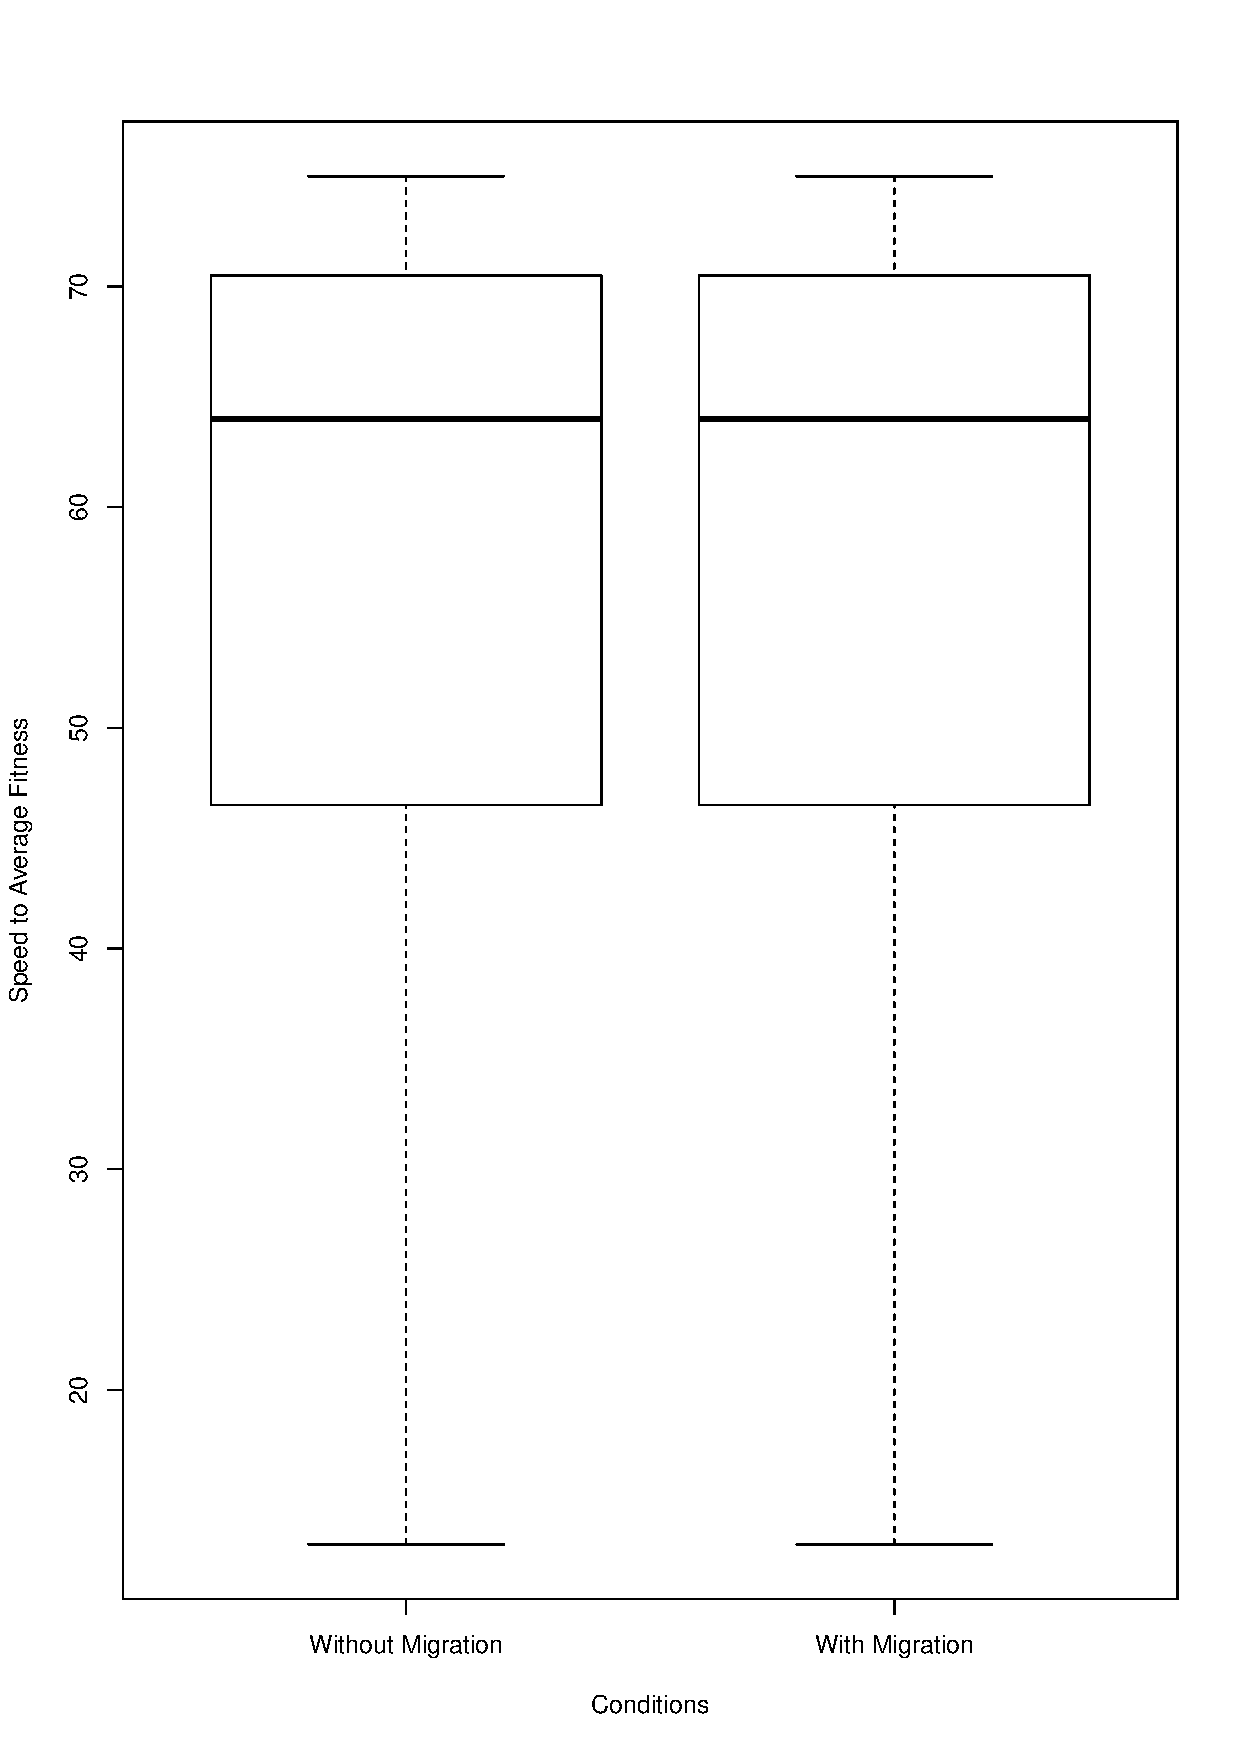
\includegraphics[width=0.8\textwidth]{../Results/boxplot_migration.pdf}
    \caption{Boxplot showing the number of generations taken to reach the average fitness of both conditions, with and without migration. When there is no migration, it takes an average of 57.4 generations (standard deviation of 15.58) to reach an average fitness value of 0.919 (standard deviation of 0.05). When migration is present, it takes an average of 57.4 generations (standard deviation of 15.55) to reach an average fitness value of 0.918 (standard deviation of 0.05).}
    \label{fig:Speed to average fit}
\end{figure}
With migration, the genetic network evolved the same as without migration. It took an average of 57.4 generations (standard deviation of 15.55) to reach an average fitness value of 0.918 (standard deviation of 0.05). The genetic network showed to evolve rapidly without migration and as well with migration as it did not affect the networks early evolution since migration did not begin till the 80th generation. The mean speeds were the same but differed was a slightly in terms of variance. This is shown in the boxplot in \textit{figure 6} to the right. The expectation was that migration would hinder the structures ability to evolve and it would take more generations to reach the average fitness. The effect of migration was seen in the variance of fitness from the plots in \textit{figure 5}. When there was migration, the fitnesses was fluctuating and going below 0.50. This was to be expected as maladaptive foreign

alleles cause the trait value and fitness to deviate from the local optimum. The variation between the different genetic structures and environmental distances was very low as conditions generated similar fitnesses and variance during periods of migration. In the periods of migration (80th generation – 700th generation), the average fitness 0.916 and a standard deviation 0.071.
